\chapter{Dynamic Gomory-Hu Tree}
    Here we seek methods to efficiently maintain a Gomory-Hu Tree also in a dynamic scenario, where the underlying graph changes over time. We consider changes in the GH tree that occurs when a concrete change occurs on a concrete edge. Similar work has been done in context of \textit{sensitivity analysis of multi-terminal flow networks} by Elmaghraby and \textit{parametric maximum flows.} by Gallo et al. and Scutella.

    \section{Finding Reusable Cuts}
    
    The main idea of this approach is to determine cuts in a given Gomory-Hu tree $T(G)$ that are still minimum separating cuts in the graph $G^{\circledU}$ after a change, and thus, can be reused for the construction of a new Gomory-Hu tree $T(G^{\circledU})$. If an old cut is not reusable with respect to this some checked vertex, then using this method it is not guaranteed that the cut won't also be reusable with respect to some other vertex. Below are some \textbf{Lemmas} and \textbf{Corollaries} to detect reusable cuts.

    \vspace{5mm}
    \noindent{\large \bf Lemma 4.1:} \textit{If $c(b,d)$ changes by $\Delta >0$, then each $\{u,v\}\in E_T$ remains a minimum u-v-cut (i) in $G^\oplus$ with cost $\lambda_G(u,v)$ if $\{u,v\}\notin \pi(b,d)$, (ii) in $G^\ominus$ with cost $\lambda_G(u,v)-\Delta$ if $\{u,v\}\in \pi(b,d)$.}

    \begin{figure}[!htb]
        \centering
        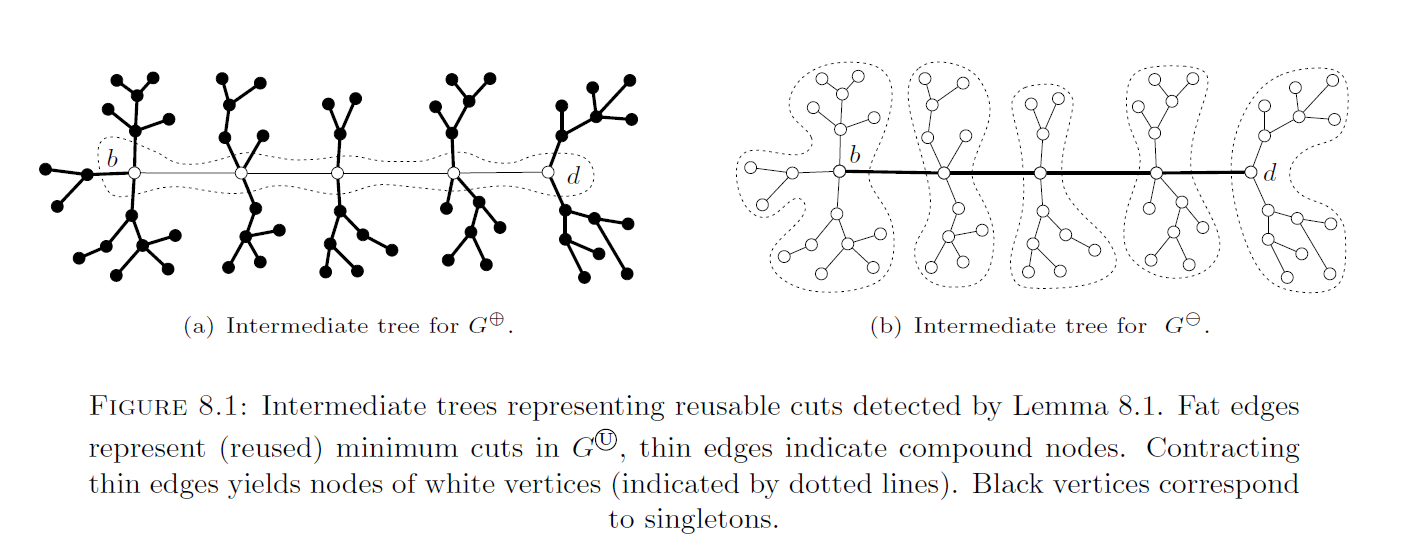
\includegraphics[width=\linewidth]{figures/G+G-.png}
        \label{GplusGminus}
    \end{figure}

    \vspace{5mm}
    \noindent{\large \bf Corollary 4.1:} \textit{If $\{b,d\}$ is newly inserted with $c^\oplus (b,d) = \Delta$ or $c(b,d)$ increases by $\Delta$, any minimum b-d-cut in $G$ remains valid in $G^\oplus$ with $\lambda_{G^\oplus}(b,d) = \lambda_G(b,d)+\Delta$.}
    \vspace{3mm}
    
    \noindent Corollary 4.1 directly allows us to use the whole Gomory-Hu tree $T(G)$ if $\{b,d\}$ is an existing bridge in $G$ with increasing cost.

    \vspace{4mm}
    \noindent{\large \bf Corollary 4.2:} \textit{An edge $\{u,v\}$ is a bridge in $G$ if and only if $c(u,v) = \lambda_G(u,v) >0$. Then $\{u,v\}$ is also an edge in $T(G)$.}

    \vspace{5mm}
    \noindent{\large \bf Lemma 4.2:} \textit{Let $\{b,d\}$ be a new bridge in $G^\oplus$. Then replacing an edge of cost 0 on $\pi (b,d)$ in $T(G)$ by $\{b,d\}$ with cost $c^\oplus (b,d)$ yields a new Gomory-Hu tree $T(G^\oplus)$.}

    \vspace{5mm}
    \noindent{\large \bf Lemma 4.3:} \textit{If $\{b,d\}$ is a bridge in $G$ and the cost decreases by $\Delta$ (or $\{b,d\}$ is deleted), decreasing all edge costs on $\pi (b,d)$ in $T(G)$ by $\Delta$ yields a new cut tree $T(G^\ominus)$.}
    \vspace{3mm}

    \noindent Lemma 4.3 allows us to easily handle edge weight decrease in bridges with 0 new flow computations.
    
    \vspace{5mm}
    \noindent{\large \bf Corollary 4.3:} \textit{Let $\{u,v\}$ denote an edge in $T(G)$ with $c_T(u,v)=0$ or an edge that corresponds to a bridge in $G$. Then $\{u,v\}$ is still a minimum u-v-cut in $G^\ominus$.}

    \vspace{5mm}
    \noindent{\large \bf Lemma 4.4:} \textit{Let $(U,V\backslash U)$ be a minimum u-v-cut in $G^\ominus$ with $\{b,d\}\subseteq V\backslash U$ and let $\{g,h\}\in E_T$ be an edge in $T(G)$ with $g,h\in U$. Then $\{g,h\}$ is a minimum separating cut in $G^\ominus$ for all its previous cut pairs within $U$.}
    \vspace{3mm}

    \noindent Lemma 4.4 allows us to reuse all edges in $E_T$ that lie on a common side of the cut.
    
    \vspace{5mm}
    \noindent{\large \bf Lemma 4.5:} \textit{Let $T_* = (V,E_*,c_*)$ denote a valid intermediate tree for $G^\ominus$, where all edges on $\pi (b,d)$ are fat and let $\{u,v\}$ be a thin edge with $v$ on $\pi (b,d)$ such that $\{u,v\}$ represents an old minimum u-v-cut in G. Let $N_\pi$ denote the set of neighbors of $v$ on $\pi (b,d)$. If $\lambda_G (u,v) \le min_{x\in N_\pi}\{c_*(x,v)\}$}, then $\{u,v\}$ is a minimum u-v-cut in $G^\ominus$.

    \section{Algorithm}
    Here we will show two update algorithms one for increase in edge costs or edge insertions and another for decrease in edge costs or edge deletion. Below in both cases it is assumed that the edge being updated is $\{b,d\}\in E$ with $\Delta >0$.

    \subsection{Increasing Edge Costs}
    If $\{b,d\}$ is an existing bridge or newly inserted bridge in $G$, then it adapts $c_T (b,d)$ according to Corollary 4.1.
    Otherwise, if $\{b,d\}$ is a newly inserted bridge in $G$, it rebuilds $T(G)$ according to Lemma 4.2. In both cases they require no new cut-computations.

    If $\{b,d\}$ is not a bridge we create the intermediate tree as in Figure~\ref{GplusGminus}(a) reusing all edges not in $\pi (b,d)$. Then as per Figure~\ref{GplusGminus}(a) we create an intermediate tree by compressing all vertices on the path $\pi (b,d)$ into a supernode and decomposing the supernode using a slightly modified version of Algorithm 2.

    \begin{algorithm}[H]
    \hrulefill
    
    \textbf{Algorithm 3:} Increase or Insert
    
    \hrulefill
    \vspace{2mm}
    
    \DontPrintSemicolon
    
    \KwIn{$T(G),\, b,d,\, c(b,d),\, c^{\oplus}(b,d),\, \Delta :=  c^{\oplus}(b,d)-c(b,d)$}
    \KwOut{$T(G^{\oplus})$}
    
    $T_{\star} \gets T(G)$\;
    
    \If{$\{b,d\}$ is a new bridge}{
        Remove an edge on $\pi (b,d)$ with cost = 0\tcp*{Lemma 4.2}
        Add edge $\{b,d\}$ with cost =$c^\oplus (b,d)$
        
        \Return{$T(G^{\oplus}) \gets T_{\star}$}
    }
    \ElseIf{$\{b,d\}$ is an existing bridge}{
        $c_*(b,d)\xleftarrow{}\lambda(b,d) +\Delta$\tcp*{Corollary 4.1}
        \Return{$T(G^{\oplus}) \gets T_{\star}$}
    }
    Construct an intermediate tree according to Figure~\ref{GplusGminus}(a)\;
    
    \Return{$T(G^{\oplus}) \gets CutTree(T_{\star})$}\;\tcp*{Algorithm 1 could also have been used}
    
    \vspace{2mm}
    \hrulefill
    \end{algorithm}

    \vspace{1cm}
    
    \subsection{Decreasing Edge Costs}
    Algorithm 4 for Decrease or Deletion of edges starts by checking if $\{b,d\}$ is a bridge, and if so then reuses the whole Gomory-He tree $T(G)$ with adapted cost $c_T(b,d)$ (Lemma 4.3). Otherwise, it constructs the intermediate tree $T_*$ as shown in Figure~\ref{GplusGminus}(b), reusing all edge on $\pi (b,d)$ with adapted costs. Then it proceeds with iterative steps where the cut pairs are chosen starting with those which have an incident vertex on $\pi (b,d)$. In this way each edge $\{u,v\}$ is found to remain valid to retain the maximal subtree (Lemma 4.4).

    \vspace{5mm}
    \noindent{\large \bf Lemma 4.6:} \textit{Let $(X,V\backslash X)$ denote a minimum x-y-cut in $G$ with $x\in X, y\in V\backslash X$ and $\{b,d\}\subseteq V\backslash X$. Let $(U,V\backslash U)$ denote a further cut. If (i) $(U,V\backslash U)$ separates $x,y$ with $x\in U$, then $c^\ominus(U\cup X,V\backslash (U\cup X))$. If (ii) $(U,V\backslash U)$ does not separate $x,y$ with $x\in V\backslash U$, then $c^\ominus(U\backslash X,V\backslash(U\backslash X)) \le c^\ominus(U,V\backslash U)$.}
    \vspace{5mm}
    
    \noindent We assume that $G$ and $G^\ominus$ are global variables. $\pi (b,d)$ is assumed to be implicitly updated at each step of the iteration. Thin edges are weighted by the old connectivity, fat edges by the new connectivity of their incident vertices. Whenever an edge is reconnected (by reconnecting one of its incident vertices), the newly occurring edge inherits the cost and the thickness from the disappearing edge. Below is the implementation of Algorithm 4:
    
    \clearpage
    \begin{algorithm}[H]
    \vspace{1cm}
    \hrulefill
    
    \textbf{Algorithm 4:} Decrease or Delete
    
    \hrulefill
    \vspace{2mm}
    
    \DontPrintSemicolon
    
    \KwIn{$T(G),\, b,d,\, c(b,d),\, c^{\ominus}(b,d),\, \Delta := c(b,d) - c^{\ominus}(b,d)$}
    \KwOut{$T(G^{\ominus})$}
    
    $T_{\star} \gets T(G)$\;
    
    \If{$\{b,d\}$ is a bridge}{
        \Return{$T(G^{\ominus}) \gets T_{\star}$}\tcp*{Lemma 4.3}
    }
    
    Construct intermediate tree according to Figure~\ref{GplusGminus}(b)\;
    
    $Q \gets$ thin edges non-increasingly ordered by their costs\;
    
    \While{$Q \neq \varnothing$}{
        
        $\{u,v\} \gets$ most expensive thin edge with $v$ on $\pi(b,d)$\;
        
        $N_x \gets$ neighbors of $v$ on $\pi(b,d)$\;
        $L \gets \min_{x \in N_x} \{c_{\star}(x,v)\}$\;
        
        \If{$L \ge \lambda_{G}(u,v)$ \textbf{or} $\{u,v\} \in E$ with $\lambda_{G}(u,v)=c(u,v)$}{\tcp*{Lemma 4.5 or Corollary 4.3}
            draw $\{u,v\}$ as a fat edge\;
            
            consider the subtree $U$ rooted at $u$ with $v \notin U$\tcp*{Lemma 4.4}
            
            draw all edges in $U$ fat; remove fat edges from $Q$\;
            
            \textbf{continue}
        }
        
        $(U, V\setminus U) \gets$ minimum $u$–$v$ cut in $G^{\ominus}$ with $u \in U$\;
        
        draw $\{u,v\}$ as a fat edge, remove $\{u,v\}$ from $Q$\;
        
        \If{$\lambda_{G}(u,v) = c^{\ominus}(U, V\setminus U)$}{\tcp*{old cut still valid}
            \textbf{goto} line 10
        }
        
        $c_{\star}(u,v) \gets c^{\ominus}(U, V\setminus U)$\tcp*{otherwise}
        
        $N \gets$ neighbors of $v$\;
        
        \ForEach{$x \in N$}{\tcp*{bend split cut by Lemma 4.6 and Lemma 2.2}
            
            \If{$x \in U$}{
                reconnect $x$ to $u$\;
            }
        }
    }
    
    \Return{$T(G^{\ominus}) \gets T_{\star}$}\;
    
    \vspace{2mm}
    \hrulefill
    \end{algorithm}
    
    \clearpage
    \section{Running Time}
    The running time of this Dynamic Gomory-Hu update procedures are clearly dominated by the computations of the new minimum separating cuts in $G^{\circledU}$. The saving in the number of flow computations for increasing edge cost and edge insertions simply depends on the length of the $|\pi (b,d)|$. Thus, in most cases saving will be quite high unless the cut structure of the underlying graph is that much degenerated that the shape of the Gomory-Hu tree is close to a linear path. In most cases, Gomory-Hu trees tend to a star-like shape, particularly for very regular graph structures. But even though star contributes for the most optimal savings in case of edge insertion, 

    \begin{wrapfigure}{r}{0.35\textwidth}
        \centering
        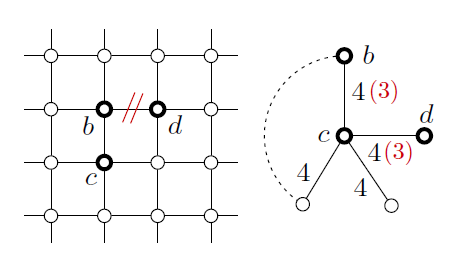
\includegraphics[width=\linewidth]{figures/Grid.png}
        \caption{Grid graph $G$ with star-shaped tree $T(G)$}.
        \label{Grid}
    \end{wrapfigure}

    it constitutes the worst-case with respect to an edge deletion or cost decrease. 
    
    Figure~\ref{Grid} shows an example based on a regular (unweighted) grid. In this example each vertex has degree 4, and we assum ethat the (global) edge connectivity is also 4. Then, the edge connectivity $\lambda_G(u,v)$ is also 4 for each vertex pair $\{u,v\}\subseteq V$, and $(\{u\},V\backslash\{u\})$ is a minimum \textit{u-v-}cut. Hence, any star with an arbitrary vertex $c$ as center and edges of cost 4 is a Gomory-Hu tree of G. Now assume the edge $\{b,d\}$ depicted in Figure~\ref{Grid} is deleted. For each vertex pair that contains at least $b$ or $d$, this decreases the connectivity to 3, however, the deletion has no effect on the connectivity of the remaining vertex pairs. Thus, decreasing the costs at the edges $\{c,b\}$ and $\{c,d\}$ in $T(G)$ would suffice to update the Gomory-Hu tree. Instead, Algorithm 4 checks each edge, apart from the two edges on $\pi (b,d)$, by computing a new minimum separating cut in $G^\ominus$. Consequently, it needs $n-3$ cut computations, which is the worst possible running time, as according to Lemma 4.3, maintaining the whole tree is possible if $\pi (b,d) = \{b,b\}$, or $\{b,d\}$ is a bridge.

    \clearpage
    \section{Limit on Fully Dynamic Algorithms}
    All known algorithms for computing Gomory-Hu Tree in a weighted graph make $\Omega(n)$ calls to an algorithm for the $s-t$ minimum cut problem. Thus, improved algorithms for constructing a Gomory-Hu Tree in a weighted graph have been corollaries of more efficient algorithms for the max. flow problem. \\
    
    Timothy G. Abbott and You Zhou proved that one of the two must happen [TY]:
    \begin{enumerate}
        \item {There are more efficient algorithms solving the Gomory-Hu problem than computing $n$ $s-t$ minimum cuts.}
        \item {There are no algorithms for dynamically maintaining the $s-t$ minimum cut in a weighted graph that are more efficient than the obvious algorithm of recomputing the cut from scratch on each query.}
    \end{enumerate}
    This is achieved using an explicit hardness relation showing that the problem of dynamically maintaining the s-t minimum cut is at least as hard as the problem of computing the  Gomory-Hu tree. This leaves open the possibility of efficient algorithms for dynamically maintaining the all-pairs $s-t$ minimum cut of a weighted graph.
    Throughout, it is assumed that all graphs are weighted graphs and all weights are non-negative. On a graph with $n$ vertices and $m$ edges, for simplicity, assume that $n = \mathcal{O}(m)$, as is the case of a connected graph.\\
    \indent
    Given a fully dynamic algorithm $A$ for the $s-t$ minimum cut problem on undirected graphs, with amortized query time $query_A(m, n)$, amortized update time $update_A(m, n)$, and initialization time $init_A(m, n)$, we give an efficient algorithm for constructing the Gomory-Hu tree on an undirected graph $G$. We assume all these time functions are monotonic and that they are bounded by a polynomial in the two inputs.
    Our data structure should support updates of adding or deleting an edge, along with adding or deleting a vertex other than $s$ and $t$ which has no edges attached to it. We will define the $s-t$ minimum cut query so that it returns the set defining one side of the cut, rather than simply the value of the cut or the edges cut.

    \vspace{5mm}
    \noindent{\large \bf Theorem 4.1:} \textit{If A is a fully dynamic algorithm for the $s-t$ mincut problem on an undirected graph, then with O(n · $query_A(m, n)+n$ · $update_A(m, n)+init_A(m, n)+n^2$) time, one can compute the Gomory-Hu tree for an undirected graph G with n vertices and m edges.}
    
    \vspace{5mm}
    \noindent{\large \bf Corollary 4.4:} \textit{If A is a fully dynamic algorithm for the s-t mincut problem, then with O(n · $query_A(m, n)+n$ · $update_A(m, n)+init_A(m, n)+n^2)$ time, one can compute the all-pairs minimum cut of an undirected graph G with n vertices and m edges.}

    \vspace{3mm}
    \noindent This shows in a strong sense, it is as hard to efficiently maintain the dynamic $s-t$ minimum cut as it is to compute the Gomory-Hu tree. 
    \clearpage
    \noindent The following theorem, equates the hardness of dynamically maintaining $s-t$ minimum cuts to the hardness of computing them in the static case, if current techniques for constructing Gomory-Hu trees from $s-t$ minimum cuts are optimal.

    \vspace{5mm}
    \noindent{\large \bf Theorem 4.2:} \textit{For any fully dynamic algorithm A maintaining the s-t minimum cut, one of the following must hold:
    \begin{enumerate}
        \item {The initialization time for A must be $\omega$(n · T(m, n)), where $T(m, n) = query_A(m, n) + update_A(m, n)$ is the larger of the update time for A and the query time for A.}
        \item {There are algorithms for computing the Gomory-Hu tree that are more efficient than O(n) s-t minimum cuts.}
        \item {A is no more efficient than computing the s-t minimum cut from scratch on each query.}
    \end{enumerate}
    }

    Since most efficient data structures do not require more than $n$ updates worth of time to initialize, Case 1 is a minor technical condition. Aside from this condition, this theorem implies that any dynamic algorithm for the $s-t$ minimum cut problem more efficient than recomputing from scratch on each query gives rise to a new, more efficient kind of algorithm for the Gomory-Hu tree problem. \\
    
    \noindent After removing the technical condition on initialization time for sparse graphs we have:
    
    \vspace{3mm}
    \noindent{\large \bf Corollary 4.5:} \textit{ For any fully dynamic algorithm A maintaining the s-t minimum cut on sparse graphs (where $m = \Theta(n)$), one of the following must hold:
    \begin{enumerate}
        \item {There are algorithms for computing the Gomory-Hu tree on sparse graphs that are more}
        \item {On sparse graphs, A is no more efficient than computing the s-t minimum cut from scratch on each query.}
    \end{enumerate}
    }

    \noindent Arikati et al. showed that one can efficiently compute the all-pairs minimum cut in sparse graphs when a certain topological property is small [Ari95], but in general there are no known algorithms for computing the Gomory-Hu tree in sparse graphs more efficiently than $n$ times the best algorithms for max flow in sparse graphs. \\
    We can similarly remove the technical condition on initialization times if we require the data structure to support bulk updates, in which a single operation supports adding or deleting a vertex along with all incident edges.

    \vspace{4mm}
    \noindent{\large \bf Corollary 4.6:} \textit{ For any fully dynamic algorithm A maintaining the s-t minimum cut and supporting bulk updates, one of the following must hold:
    \begin{enumerate}
        \item {There are algorithms for computing the Gomory-Hu tree that are more efficient than computing O(n) s-t minimum cuts.}
        \item {A is no more efficient than computing the s-t minimum cut from scratch on each query.}
    \end{enumerate}
    }

    % Developing efficient algorithms for dynamically maintaining the Gomory-Hu tree (or showing that they cannot exist) would be a good direction for future investigation.